%
%
%

\chapter{Search and Optimization with python}

\section{Problem Statement and Learning Objectives}

The problem of this chapter is to find a good set of PID control parameters ($K_P,K_I,K_D$) by searching the 3D space created by those values.
A key aspect of this search is careful definition of ``good''.  We will focus on  the following aspects of performance
{\it when the system has a step input}.
with
\begin{itemize}
\item  $T_S$ (settling time)
\item $\%OS$ (percent overshoot)
\item $SSE$ (Steady State Error)
\item $Cu_{max}$, the amount of effort applied by the controller to the plant (related to energy consumption).
\end{itemize}

In each case we will find the controller which achieves response closest to the desired value.
We will introduce and use a set of python routines which simply search a 3D space by nested iteration.

Upon completing this chapter, the successful student will be able to:

\begin{itemize}
  \item Take an initial rough design of PID parameters, and, using a specific computational tool, refine it to achieve one or more performance specifications without simplifying assumptions.
  \item Manage the trade-off between accuracy and computation time to get results in an efficient manner.
\end{itemize}





%%%%** Section 2.2
\section{Overview}

We will use two python scripts to search the three dimensional space defined by
\[
K_P, K_I, K_D
\]
for the ``best'' design.  We can define the best design according to various {\bf Performance Criteria}.
We will look at the most common performance criteria, and one additional criterion: control effort which
has large practical effects on system designs.
s
\begin{itemize}
  \item Settling Time, $T_S$
  \item Percent Overshoot, $\%OS$
  \item Steady State Error, $SSE$.
  \item Control Effort, $cu$.
  \item Gain Margin, $gm$.
\end{itemize}

We supply a set of python methods or code which can analyze a step response and determine $T_S$ and $\%OS$.
The functions are

\begin{itemize}
  \item {\tt ts = settletime(t,y)}
  \item {\tt o = PCTovershoot(t,y)}
  \item {\tt sse =steady\_state\_error(t, y) }
  \item {\tt Cu = ctl\_eff(sys) }
  \item Gain margin is computed by the {\tt python} function {\tt margin()}.
\end{itemize}

Steady state error is approximated by the final value in the step response, and we compute maximum control effort by simulating the system again using the equation in Section \ref{CtlEff}.	%<h>



%\end{frame}  %%%%%%%%%%%%%%%%%%%%%%%%%%%%%%%%%%%%%%



%%%%** Section 2.3
\subsection{Performance Functions}
%\begin{frame}

The python method {\tt cost\_pid()} uses several functions which compute the performance measures from the step response.

{\bf Settling Time: $T_S$}

Settling time ($T_S$) is the time from the start of step input until the response stays within 2\% of its final value
(not necessarily the {\it desired} final value if SSE is non zero).	%<h>

{\bf Percent Overshoot: $POS$}

$POS$ is the percentage by which the step response exceeds its final value.


{\bf Steady State Error: $SSE$}

$SSE$ is the difference between the final value of the step response and the amplitude of the input step (we use 1.0).

{\bf Actuator Effort: $U_{MAX}$}

Actuator effort (same as control effort) is the amount of output from your actuator which is given to the plant.  A controller design must achieve its step response specs without requiring excessive output from its actuator.   By including actuator effort into the cost function, we make sure that the controller we design is practical.   The measure of actuator effort will be the peak value during the simulation time, $\max{u(t)}$.

{\bf Gain Margin: $gm$}

Gain Margin is described in Section \ref{GainPhaseMargins}.   In brief, if a system has gain margin $GM$ (usually expressed in $dB$), then the magnitude of the loop gain ($|CPH(s)|$) can be increased by that amount of gain while still remaining stable.  For example, for a gain margin of $20dB$, we can add $+19dB$ of gain to $CPH(s)$ and the system will still be stable (but the new gain margin will be only $1dB$).

We will specify a target or ``desired value'' for each performance measure, for example $T_{sd} = 0.25$ means we set a goal to find a
design with a settling time of $0.25$sec.  We will measure one aspect of how good is our design by minimizing the difference between
our design's performance and the desired value, in this case
\[
|(T_s - T_{sd})|
\]
If we only care about settling time, then our goal is to minimize this quantity.


%%%%** Section 2.4
\subsection{Weights}
%\begin{frame}

We need a  way to combine the different performance measures into a single ``cost''.  We can define ``cost'' as the absolute difference between the performance and
our specs. We will adjust the system to minimize cost, but different performance criteria may conflict with each other\footnote{A classic example: Powerful cars (V8 engine = high performance) get bad gas milage (15mpg = high gas cost).}.
For example, what if we get really good settling time, but horrible overshoot?  We need a score which potentially combines all four of our measures in to a single number.   We will use a combined score as follows:	%<h>

% Let's combine these scores into one

\[
S = w_1 \times |T_s-T_{sd}| + w_2 \times |\%OS-\%OS_d| + w_3 \times |SSE-SSE_d| + w_4 \times (\max(u(t))) + w_5\times |gm-gm_d|
\]
where $w_i$ are weights which add up to 1.  We define the {\it weight vector} to be
\[
w = \begin{bmatrix} w_1 \\ w_2 \\ w_3 \\ w_4 \\w_5 \end{bmatrix}
\]
There is one remaining problem with this scheme which is that the different performance measures have different numerical values and units which can mess up the weights.   For example, since $Ts$ might be only 0.2, if all weights are equal, it would not count much in the final score if $\max(u(t)) = 2000$.  To equalize the influence of each performance criterion, we will normalize the difference as follows:


\[
S = w_1 \times |T_s-T_{sd}|/T_{sd} + w_2 \times |\%OS-\%OS_d|/\%OS_d + w_3 \times |SSE-SSE_d|/SSE_d + w_4 \times \max(u(t))/u_{max} + w_5\times |gm-gm_d|/gm_d
\]

or more compactly
 \[
 S = \Sigma_i w_i \frac {C_i}  {C_{iD}}
 \]
 where $C_{iD}$ is the desired value for cost component $C_i$.

Generally all the specifications will be given as inputs to the design problem.
$u_{max}$ must be set by the actuator (motors, hydraulics, etc) specification.  Alternatively, if the actuator is not specified yet, we can experiment to see what kind of actuator is necessary for a give set of specs.

The result, $S$, can be viewed as a ``Cost'' of a given design, which is zero when all the specifications are met.

Now the question is which weights to choose?    This is another difficult question.  However, since we are searching the entire design space, we do not necessarily have to choose a single weight scheme.   We could define several and find the best design for each weight vector in a single pass through the space.  In our approach, we keep track of several weighting schemes simultaneously.  For example, we can track the best gains we find for each of these different weight vectors as we search.
\vspace{0.1in}

\begin{center}
\begin{tabular}{|l|c|c|c|c|} \hline
Scheme Name	&   $ w_1$	& $w_2$	& $w_3$ & $w_4$ \\ \hline
Settling Time  &   1    &  0    &   0   &  0  \\ \hline
Overshoot      &   0    &  1    &   0   &  0  \\ \hline
Steady State Error &  0  &  0    &   1   &  0  \\ \hline
Control Effort   &  0  &  0     &   0   &  1  \\ \hline
Balanced        &   0.25 & 0.25 & 0.25 & 0.25 \\ \hline
\end{tabular}
\end{center}

%%%%** Section 2.5
\subsection{Gain Space Searching and Optimization}\label{searchrange}
%\begin{frame}


As an example, consider a controller having two parameters, $P_1, P_2$.  For each point $\{P_1 , P_2 \}$, there is a certain step response and a certain resulting cost.  In Figure \ref{CostFunc}, the two values, $P_1, P_2$ form a plane, and we can represent the cost at each point in the third axis.   In the illustration, the point $\{m,n\}$ represents the lowest value of cost over the whole plane.  A simple function like a parabola can usually be easily optimized, however the cost function for step responses is not so simple, and is not known analytically.
Our strategy will be to
\begin{enumerate}
  \item Choose initial values for the three gains $K_P, K_I, K_D$.
  \item Define a range of each value to search.
  \item Define how many discrete values to search for each gain, $Nvals$
  \item Try every combination of values and find those which produce the ``best'' step response.
\end{enumerate}

%\end{frame}  %%%%%%%%%%%%%%%%%%%%%%%%%%%%%%%%%%%%%%%%%%%%%%%%%%%%%%%

%\begin{frame}
%\frametitle{Example}

%%%%** Figure 9
\begin{figure}\centering
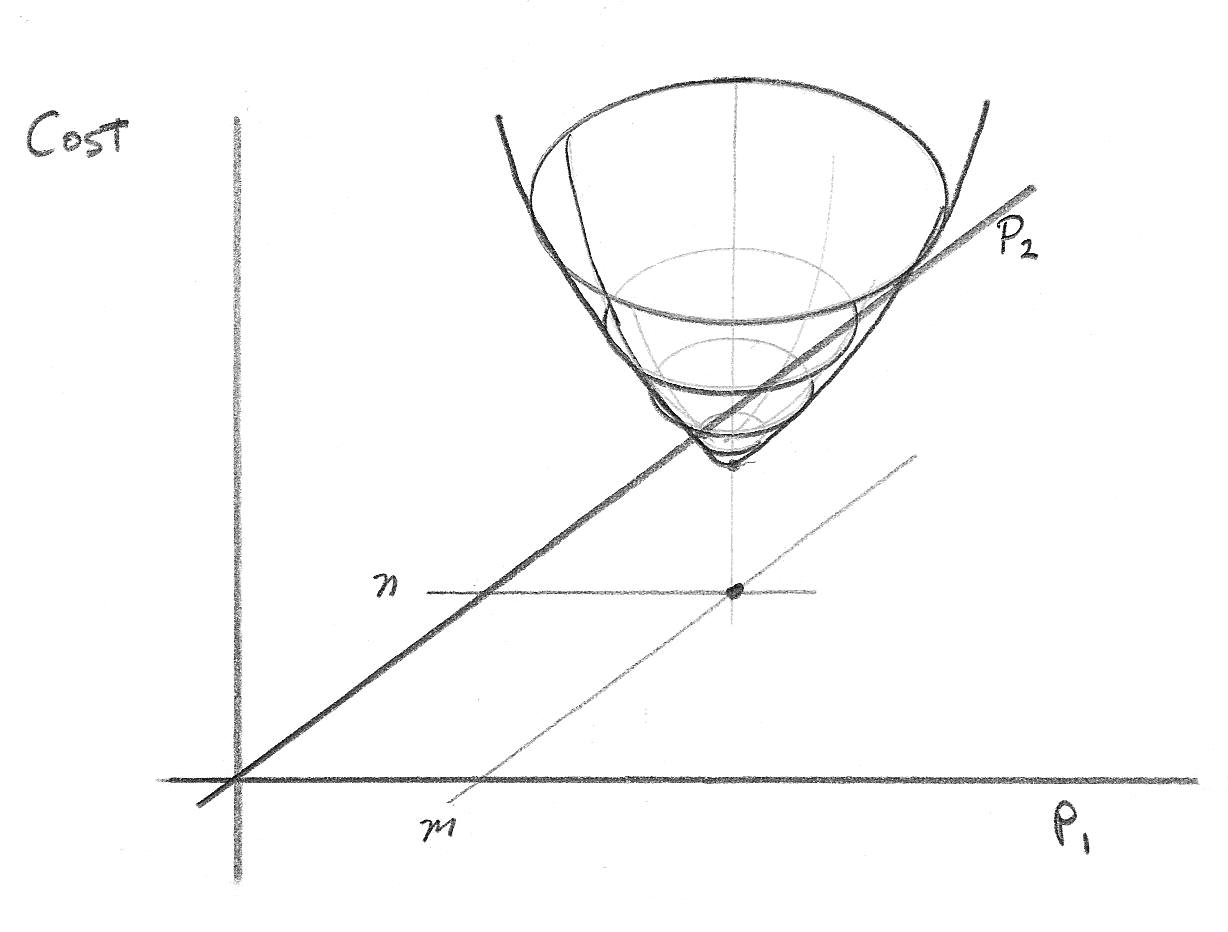
\includegraphics[width = 3.5in]{figs09/00648.png}
\caption{Idealized cost function which has a minimum (optimum) at $P_1=m, P_2=n$.}\label{CostFunc}
\end{figure}




%\end{frame}  %%%%%%%%%%%%%%%%%%%%%%%%%%%%%%%%%%%%%%%%%%%%%%%%%%%%%%%


%\begin{frame}[containsverbatim]

	%<*h>
In our PID control design problem, the three parameters could be thought of as forming a 3 dimensional space.  Each controller is a single point in that space.

The simplest optimization method is to discretize the parameters and search all of the possible combinations.
When the space of all parameter values gets very large, it can be too computationally expensive to try all the possible points in parameter space.  In this case special algorithms are used or mathematical assumptions are made to speed the process.
In our PID control design however we have only a 3 dimensional parameter space and simulation of step responses is sufficiently fast that we can do the brute-force exhaustive search in a reasonable time:
	%<*>


\begin{verbatim}
for Kp in range(kmin, kmax + dk, dk):
  for Ki in range(kimin, kimax + dki, dki):
    for Kd in range(kdmin, kdmax + dkd, dkd):

               *** simulation and optimization code here

\end{verbatim}



%\end{frame}  %%%%%%%%%%%%%%%%%%%%%%%%%%%%%%%%%%%%%%%%%%%%%%%%%%%%%%%

%\begin{frame}


The algorithm will loop through a set of values for each of the three gains and keep track of which one produced the highest performance by each of the weight schemes.

{\bf Search Range}  We will define our search range in terms of the center value and a multiplicative range $r$. If our nominal value is $K_0$, then
\[
K_{min} = K_0/\sqrt{r} \qquad  K_{max} = \sqrt{r}\times K_0
\]
  With this scheme,
\bq\label{ranger}
K_{max} = rK_{min}
\eq


This method is illustrated below with respect to the nominal (center) value.	%<h>
\begin{center}
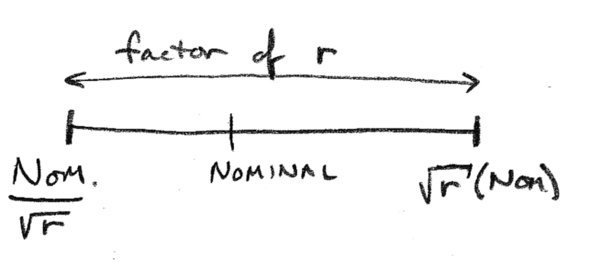
\includegraphics[width=50mm]{figs11/00615a.png}
\end{center}

Other search range methods are possible but  note that this approach will never generate negative gain values (which are not allowed for PID controllers anyway).	%<h>

It can be tricky to know a good initial value for the gains $K_p,K_i, K_D$.   Depending on the problem they can range from much less than 1 to hundreds.   One computer-only approach, is to start your search over a wide range and then narrow it down on subsequent searches.  However this takes many optimization runs to find a good answer.   A better approach is to do a rough manual PID design (Section \ref{manualPIDdesign}).  The result of your manual design is a good starting point.

{\bf Search size} Next we choose how many discrete values we will try within the search range for each of the three gains, $Nvals$.  The number of simulations we must run is then $Nvals^3$.    My computer can   do about 500-1000 simulations per minute in python.	%<h>


%%%%** Section 2.6
\subsection{Range Saturation}

%\begin{frame}
% <s>\frametitle{Range Saturation}
One way this scheme can fail is if an optimium exists outside the range of parameters that you specify.  In this case, the algorithm is likely to find a value at the extreme of its search range.  If the algorithm reports a value at the extreme of its range, this fact is annouced for you in the output and it is then a good idea to run the simulation again, centering on the extreme of the output range.   The algorithm will indicate that its best weighted performance score was found at the edge of its ``box'' by printing, for example, {\tt kp min}.  This would mean that the value of $K_P$ which yielded the best value was at the edge of the search space.	%<h>


%%%%** Figure 10
\begin{figure}\centering
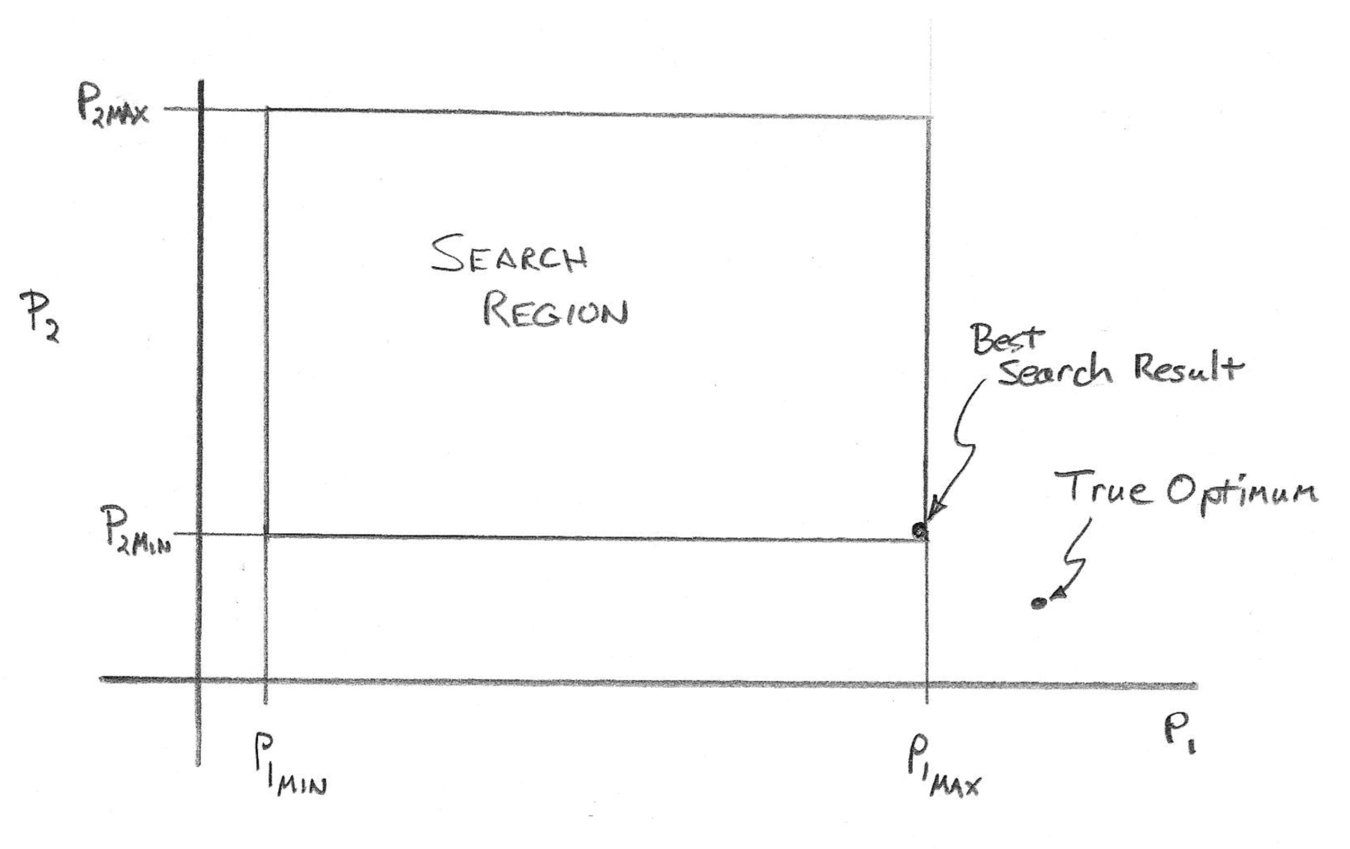
\includegraphics[width=4.5in]{figs10/00649a.png}
\caption{Search range does not contain the true optimum of the function and finds a minimum in one corner.}\label{rangesat}
\end{figure}


Figure \ref{rangesat} shows a two-dimensional example in which the search has saturated its range at $P_{1max}$ and $P_{2min}$.  The actual best design is outside the search range and the search only found the closest point it could.   Clearly we should move the search range to the lower right and run again.   Note that we have made an assumption about the cost function in doing this, what is that assumption?	%<h>


%\end{frame}   %%%%%%%%%%%%%%%%%%%%%%%%%%%%%%%%%%%%%%%%%%%%%%%%%%%%%%%%



%%%%** Section 3
\section{Using the python packages}

%\begin{frame}
I have supplied two python files:
\begin{itemize}
  \item {\tt setup.py}
This file contains code to initialize the simulation.  In here you define your system, define your specifications (requirements), and your initial values and search ranges.  Make a new copy of this, with a new name, for each problem you work on.
%   \item {\tt stepperf.py}
% This file contains functions to evaluate $T_S$ and $\%OS$.	%<h>
  \item {\tt optigain.py}
  This file searches for the best design according to different weight schemes and saves the best ones.  All ``best'' designs are plotted at the end of the search.  This function takes on the order of minutes to complete ($N$ is the current version number).
\end{itemize}

%\end{frame}   %%%%%%%%%%%%%%%%%%%%%%%%%%%%%%%%%%%%%%%%%%%%%%%%%%%%%%%%


%
%
% %%%%** Section 3.1
% \subsection{optivis.py}
%
% %\begin{frame}
% An experiental script is available to visualize the search space to make it easier to narrow your search.  {\tt optivis.py} can be substituted for {\tt optigain2.py} in your startup script to experiment with this feature.	%<h>
%
% {\tt optivis.py }
%
% \begin{itemize}
%     \item Visualize the search space
%     \item help to locate good start point(?)
%     \item still experimental
% \end{itemize}



%%%%** Section 4
\section{Solving Design Problems}

%\begin{frame}
%\frametitle{Solving Design Problems}

Here is the procedure to use these tools to solve a design problem.
First, collect your information:
\begin{itemize}
  \item  Plant model (as in previous chapters). (Know the gain, poles, and zeros of your plant)
  \item  Required step response specs:  \% Overshoot, Settling Time (2\%), SSE (usually 0), and Gain Margin.
  \item  For Control effort, you need the Actuator Effort normalization constant, $u_{max}$ (sometimes also called $cu_{max}$.   If you don't care about actuator effort, set the constant to a really huge number.
\end{itemize}

Then follow these steps:	%<h>

\begin{enumerate}
  \item Copy the file {\tt setup.py} to a new file such as {\tt setup\_problem5.py}.
  \item Open the new file in a text editor or jupyter notebook.
  \item Set the simulation time where it says {\tt tmax = }.
This is how long the step response will be simulated and it should be about 5 times your desired settling time: $tmax \approx 5T_{sd}$.
  \item Enter the transfer function of the system you wish to control (plant) (not your PID controller) under the comment {\tt /\#plant transfer function}.
  \item Identify the highest frequency pole or zero in your plant.  Multiply it by 20 and set the {\tt pp} variable to that value. This is the controller normalization pole, $pp$.
  \item Edit the desired performance specs below their comment.  Note that 5\% overshoot should be entered 1.05, and gain margin should be entered in $dB$.
  \item Enter {\tt nvals}.  This is the number of values which will be tried of each parameter.
Note that the total search time will be proportional to {\tt nvals}$^3$ so keep this below 10 until you get a feel for how long the searches take.
  \item Enter {\tt scale\_range}.  This is the range, $r$, from Equation \ref{ranger}.
  \item Save your file.
  \item Within python environment start {\tt setup\_problem5.py} to initiate the search.
\end{enumerate}


%%%%** Section 5
\section{Description of Software Operation}

%\begin{frame}
Please refer to the code listings for each script file.

\subsection{setup.py}

We start with some code which looks for a stored file ({\tt simrate\_optigain.txt}) which tells how fast
the simulations are running on the current machine.  This is used to predict runtime for the user (If the file's
not there, we have a default which is replaced after the first run.)

Next, after setting up $s$, we define the plant transfer function.  Edit your numerator and denominator polynomials here or use the $s$ we just defined
to write out the plant transfer function directly.

Next we set up our initial values (geometric center of the search cube).

After that
we enter specifications for $T_S$({\tt tsd}), $\%OS$ ({\tt pod}), etc.   We also enter our maximum actuator output ($cu_{max})$.


$T_{max}$ and $dt$ are set next because they depend on the details of the problem.  For example, if
the expected $T_S$ is $0.1sec$, we should not simulate for 10 minutes.   Typically, set
$T_{max}$ to about 4-5 times the $T_S$ specification.   Set $dt$ to have at least 100 simulation
steps during the $0-T{max}$ interval.


Next we enter search parameters such as the  number of values we should search.  The more values ({\tt nvals}) that we select, the more accurate our result.  However computation time is proportional to {\tt nvals}$^3$.
Finally, we  enter the {\tt scale\_range} factor ($r$) described in Section \ref{searchrange}.



\subsection{optigain.py}
This code starts by setting up the time vector, {\tt t}, and storing the start time of the simulation run (in seconds).

The function {\tt [ts, po, cu, gm, y] = costPID(plant, Kp, Ki, Kd)} accepts the plant and the three PID controller parameters, and returns the settling time, {\tt ts},  the percent overshoot, {\tt po}, the max control effort, {\tt cu}, the gain margin {\tt gm}, and the step response, {\tt y}.   {\tt y} is a vector of the same length as {\tt t} which contains the output of the control system with a unit step input, $Y(t)$.  This will be used to evaluate the cost of  each controller in the search.

After definition of {\tt costPID()} (we will return to it shortly), we set up weight schemes so that we can store the ``best'' controller by several different definitions.  Each weight scheme has a name such as ``Overshoot''.

After we initialize the storage and set up the limits for each parameter, we start searching in the ``Main Loop''.
Three {\tt for} loops iterate through the 3D parameter space. For each point, we have values of {\tt Kp, Ki, Kd} to test with {\tt costPID()}.

Now we'll look at the workings of {\tt costPID()}.
After generating the new controller and the new loopgain ($CPH(s)$), we use the python {\tt ctl.margin()} function to get the gain margin from the loop gain, $CPH(s)$, which includes
everything around the loop.

Sometimes the combination of gains we have picked results in an unstable system.
There is no point in simulating and evaluating the responses if the system is going to go unstable (because the gains have moved closed loop poles into the right half plane).
For each set of gains, {\tt costPID}
first determines stability by getting the characteristic polynomial, solving the roots, and then checking for any positive real parts.
If there are any poles with positive real parts, the simulation step is skipped and artificially high-cost,
``flag'', values (e.g. 999) are returned for the costs.
Assuming the system is stable, then the system and control effort are simulated ({\tt csim()}) and the performance measures are computed.

Now we return back from {\tt costPID} to the ``Main Loop''.   If the system was stable, the different weighted scores are compared with the stored best ones and if better they replace the previous value so that the best controller (i.e. best set of values for $K_p, K_I, K_D$) is saved for each different weighted score.

Finally, the results are printed and plotted for the user.



%%%%** Section 6
\section{Example Design}


(This problem is Example 9.5 from Nice, page 483).
% The output of this example was generated before the control effort and gain margin
% computations were added to {\tt optigain.py}.


{\bf Problem: }
Design a PID controller for a system where the plant is:

\[
P(s) = \frac{22.5(s+8)}{(s+3)(s+6)(s+10)}
\]

Step response must have
\[
T_S = 0.55 \mathrm{(sec)} \qquad  \%OS = 20\% \qquad    SSE = 0
\]


{\bf Solution Procedure}

Rename {\tt setup.py} to {\tt setup10p6.py} (for this example)
to input the plant and the performance specifications above.
Set the initial values of $K_P= K_I=K_D=1$
(note {\tt K1, K2, K3 } are used in some parts of the
code instead of $K_P, K_I, K_D$).

Some initial work for this system gave a starting point of
 \[
 K_P = 15, K_I= 15, K_D=0.25
 \]

Set {\tt Nvals = 12}  (the code actually searches {\tt Nvals+1} values each to hit both ends of the
search range) and start close to this value: {\tt scale\_range = 5}.

{\bf Search 1}

Using the command line or your Jupyter Notebook, run {\tt setup10p6.py'}.
The script will call {\tt optigain.py} to perform the search of $13^3 = 2197$
controllers with the different values of the three gains, and finds the
combination of gains that gives the best step response for each weight scheme.

At the end of the search the five best step responses
(according to your 5 weight schemes)
are plotted automatically and the gains are reported on the console.

Our first results are somewhat promising (Figure \ref{PIDsearchV1x5}).
A 6th weight vector was added ({\tt W\_BH}) which weights settling time and percent overshoot
equally and ignores the others.

%%%%** Figure
\begin{figure}\centering
  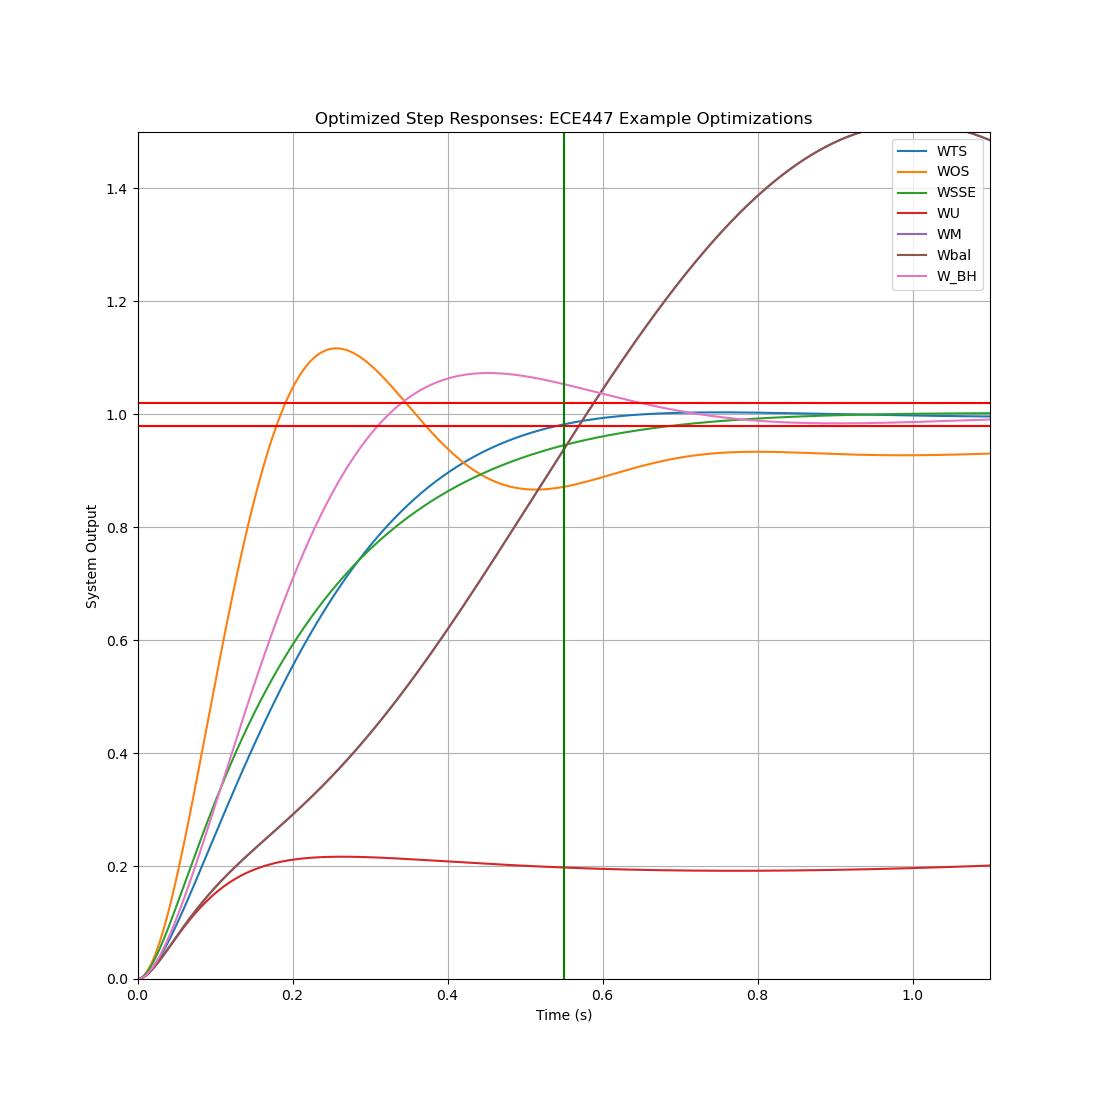
\includegraphics[width=4.5in]{figs10/S43Q01.png}
  \caption{Results of our first PID search.   There are 6 step responses.
  Red horizontal lines are shown for the $T_S$ window which must be entered by
  $t=0.55$ (green line)}\label{PIDsearchV1x5}
\end{figure}

\begin{verbatim}
  Checking Search Boundaries ( Wbal )
  Search boundary reached: Kd min

  Search Time:  3.63 minutes.  N sims = 9261  (2804129.0 ticks/min)
  Do you want to see results printout? <CR>
  Goals:
  tsd   : 0.55   pod   : 20.0   ssed  : 0.0   cu_max: 100000   gm_db : 10.0


  Reporting:  WTS
  [Ts = 0.550           Kp:  7.270  Ki: 29.907  Kd:  0.559
  Settling Time:  0.550  Overshoot: 15.539 %   SSE:  0.001 Ctl Effort: 22.361   Gain Marg:   80.0 dB  ]


  Reporting:  WOS
  [Overshoot = 20.00    Kp:  6.708  Ki: 17.027  Kd:  0.294
  Settling Time:  0.668  Overshoot: 19.994 %   SSE:  0.000 Ctl Effort: 11.746   Gain Marg:   80.0 dB  ]


  Reporting:  WSSE
  [SSE = 0.00           Kp:  7.880  Ki: 20.000  Kd:  0.439
  Settling Time:  0.412  Overshoot: 16.004 %   SSE:  0.000 Ctl Effort: 17.565   Gain Marg:   80.0 dB  ]


  Reporting:  WU
  [Control Effort Max = 100000.00 Kp:  6.708  Ki:  8.944  Kd:  0.112
  Settling Time:  1.099  Overshoot: 28.884 %   SSE:  0.028 Ctl Effort:  5.997   Gain Marg:   26.5 dB  ]


  Reporting:  WM
  [Gain Margin = 10dB   Kp: 13.840  Ki: 12.341  Kd:  0.131
  Settling Time:  1.099  Overshoot: 58.156 %   SSE:  0.048 Ctl Effort: 11.266   Gain Marg:   10.0 dB  ]


  Reporting:  Wbal
  [Balanced             Kp: 11.783  Ki:  9.694  Kd:  0.112
  Settling Time:  0.944  Overshoot: 44.784 %   SSE:  0.003 Ctl Effort:  9.746   Gain Marg:   11.5 dB  ]


  Reporting:  W_BH
  [BH_bal               Kp:  9.256  Ki: 20.000  Kd:  0.439
  Settling Time:  0.547  Overshoot: 19.753 %   SSE:  0.001 Ctl Effort: 17.565   Gain Marg:   80.0 dB  ]
  \end{verbatim}

Looking at the printed outputs, we get a report of the best results for each weight vector.  From the top, for example is the search
that weights {\it only} settling time.   With the gains $K_p=7.3,
K_I = 29.9, K_D = 0.56$, $T_S= 0.55$.  Exactly at
the goal.  Overshoot was a bit below the spec (which could be
good actually depending on the application).
Steady state error is little or none (excellent for most applications).
Peak control effort is about 12
- we can match this with motor specifications.  Finally the gain margin of 80dB is excellent:
there seems to be a low chance of component tolerances or
plant wear and tear changing the model enough to drive it unstable.

If we try to achieve all our specs, let's look at the Balanced
report ({\tt Wbal}).  That one has slower settling, too much overshoot and a worse but still good SSE.

The final weight result ({\tt W\_BH})
considers only
the $T_S (60\%)$ and $\%OS (40\%)$ specs, and SSE and Gain Margin are solid.

This is a really nice result overall but control effort is about double the
Balanced result and we reached a search boundary ($K_{dmin}=0.112$) on the balanced weights

As a result, let's do

Search 2:

We will choose gains between the {\tt Balanced} and {\tt W\_BH} gains:

 \[
 K_p = 10.0, \; K_i = 15, \; K_d = 0.2
 \]

and reduce the search range to 2.

We are still hitting a search boundary so this time we will take the balanced gains
below, and just reduce $K_D$

\begin{verbatim}
Reporting:  Wbal
  [Balanced             Kp: 11.892  Ki: 12.613  Kd:  0.141
  Settling Time:  0.930  Overshoot: 44.141 %   SSE:  0.000 Ctl Effort:  9.897   Gain Marg:   13.5 dB  ]
\end{verbatim}

Search 3:

\[
K_p = 10.0, \; K_i = 15, \; K_d = 0.05
\]




---
This is a pretty good compromise between overshoot close to 20\%
and $T_S$ close to 0.55.   SSE is great, Gain margin is great,
and we now now what amount of control effort is to be expected
for this performance.

The step response we get using the balanced gains is given
in Figure \ref{FinalDesignSim}:

%%%%** Figure 12
\begin{figure}\centering
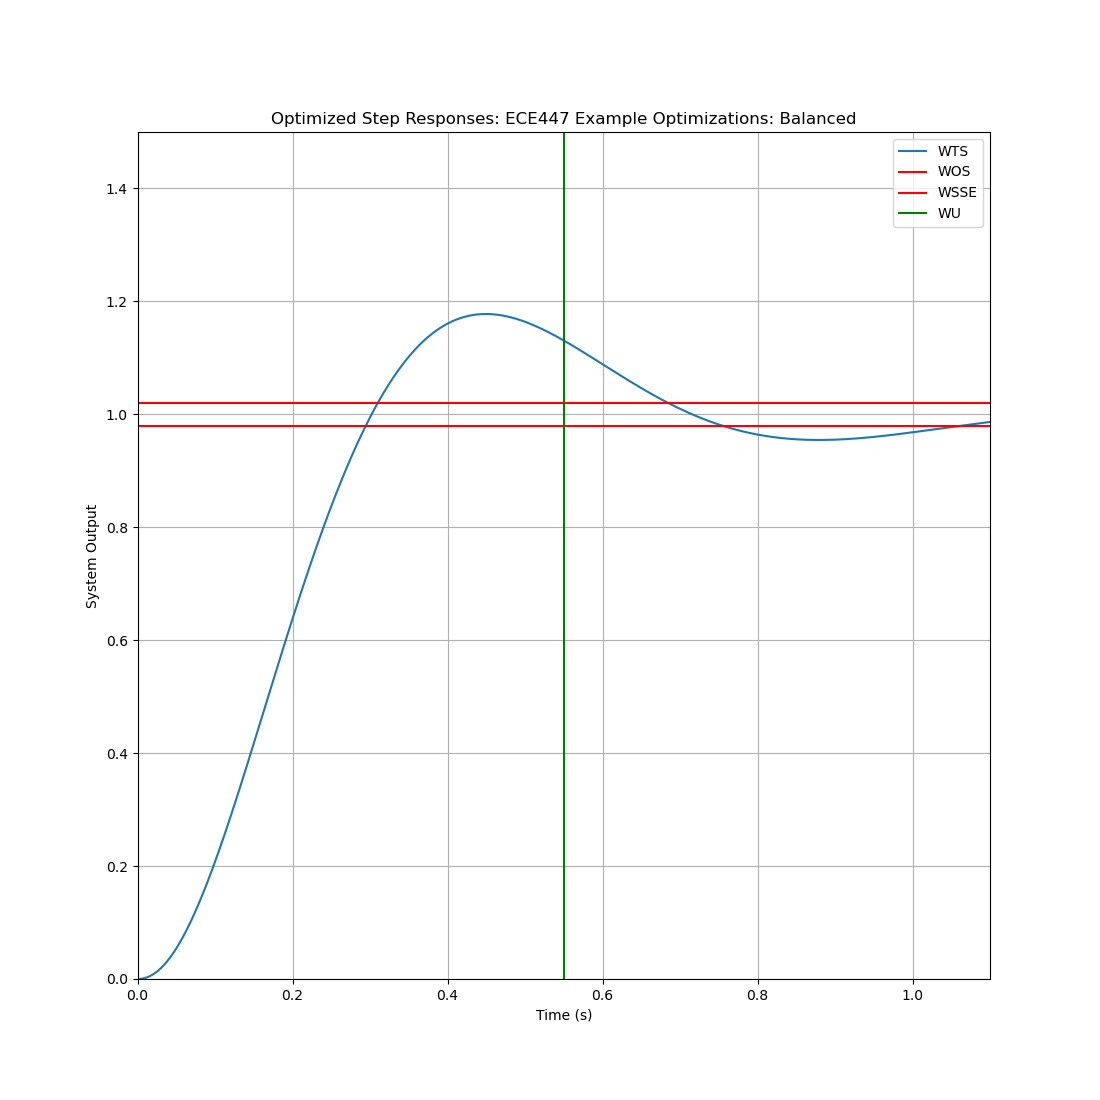
\includegraphics[width=4.5in]{figs10/S43Q02.png}
\caption{Simulation result of final design.}\label{FinalDesignSim}
\end{figure}
 %%%%%%%%%%%%%%%%%%%%%%%%%%%%%%%%



% \section{Summary of Notation}

